\documentclass[aspectratio=169, 11pt]{beamer}

% ── Theme & Colors ──────────────────────────────────────────
\usetheme{Madrid}
\usecolortheme{default}

\definecolor{deepblue}{RGB}{20, 66, 114}
\definecolor{accentblue}{RGB}{41, 128, 185}
\definecolor{lightblue}{RGB}{214, 234, 248}
\definecolor{accentorange}{RGB}{230, 126, 34}
\definecolor{accentgreen}{RGB}{39, 174, 96}
\definecolor{darkgray}{RGB}{52, 73, 94}
\definecolor{lightgray}{RGB}{236, 240, 241}
\definecolor{accentred}{RGB}{192, 57, 43}
\definecolor{softpurple}{RGB}{142, 68, 173}

\setbeamercolor{structure}{fg=deepblue}
\setbeamercolor{palette primary}{bg=deepblue, fg=white}
\setbeamercolor{palette secondary}{bg=accentblue, fg=white}
\setbeamercolor{palette tertiary}{bg=deepblue!80, fg=white}
\setbeamercolor{frametitle}{bg=deepblue, fg=white}
\setbeamercolor{title}{fg=white}
\setbeamercolor{block title}{bg=accentblue, fg=white}
\setbeamercolor{block body}{bg=lightblue!30}
\setbeamercolor{block title alerted}{bg=accentorange, fg=white}
\setbeamercolor{block body alerted}{bg=accentorange!12}
\setbeamercolor{block title example}{bg=accentgreen, fg=white}
\setbeamercolor{block body example}{bg=accentgreen!10}
\setbeamercolor{item}{fg=accentblue}

\setbeamertemplate{navigation symbols}{}
\setbeamertemplate{footline}{%
  \hfill\insertframenumber/\inserttotalframenumber\hspace*{4pt}\vspace{2pt}%
}

\usepackage{tikz}
\usetikzlibrary{arrows.meta, positioning, shapes.geometric, fit, backgrounds}

% TikZ block styles
\tikzset{
  core/.style={rectangle, rounded corners=3pt, draw=darkgray, fill=lightgray,
               text width=2.4cm, align=center, font=\scriptsize, minimum height=0.9cm},
  toolb/.style={rectangle, rounded corners=3pt, draw=accentgreen!80!black, fill=accentgreen!12,
               text width=2.7cm, align=center, font=\scriptsize, minimum height=0.8cm},
  apib/.style={ellipse, draw=softpurple, fill=softpurple!12,
               text width=2.2cm, align=center, font=\scriptsize, minimum height=0.7cm},
  stage/.style={rectangle, rounded corners=4pt, draw=deepblue, fill=lightblue!40,
               text width=2.5cm, align=center, font=\scriptsize, minimum height=1.5cm},
  arr/.style={-{Stealth[length=2.2mm]}, draw=darkgray, line width=0.7pt},
}

% ── Title ───────────────────────────────────────────────────
\title[Agentic Enzyme Discovery]{An Agentic Framework for Enzyme Discovery}
\subtitle{Autonomous, LLM-driven discovery of candidate enzymes for non-natural reactions}
\author{Biochemical Agent}
\institute{Argonne National Laboratory}
\date{\today}

\begin{document}

% ── 1. Title ────────────────────────────────────────────────
\begin{frame}[plain]
  \titlepage
  \begin{center}
    \footnotesize\color{darkgray}
    \emph{Given a target reaction, the agent reasons, searches, and ranks
    candidate enzymes --- with no human in the loop.}
  \end{center}
\end{frame}

% ── 2. The problem ──────────────────────────────────────────
\begin{frame}{The problem: enzymes for reactions nobody catalogued}
  \begin{columns}[T]
    \begin{column}{0.54\textwidth}
      \textbf{Input:} a target transformation \\[-2pt]
      {\footnotesize (substrates + ``what bond is made/broken'')}

      \medskip
      \textbf{Output:} a \emph{ranked, evidence-backed} list of enzymes that
      could plausibly catalyze it.

      \bigskip
      \begin{alertblock}{Why this is hard}
        \footnotesize
        The best catalysts for a \emph{non-natural} reaction are often
        \textbf{promiscuous} enzymes: the right catalytic machinery, but the
        \emph{wrong or missing annotation}.
        \begin{itemize}\setlength\itemsep{1pt}
          \item EC / keyword search finds them by \emph{native} function $\Rightarrow$ misses them
          \item The true catalyst may be an unreviewed (TrEMBL) protein named only in a paper's full text
        \end{itemize}
      \end{alertblock}
    \end{column}
    \begin{column}{0.46\textwidth}
      \begin{block}{Guiding insight}
        \footnotesize
        \textbf{Promiscuity conserves catalytic \emph{machinery}, not
        \emph{substrate}.}
        \begin{itemize}\setlength\itemsep{2pt}
          \item \textbf{Recall} must run on \emph{mechanism} ---
                fold / domain / active site --- which survives the annotation gap.
          \item \textbf{Substrate fit} is the \emph{discriminator}: it belongs in
                \emph{ranking}, never as a recall filter.
        \end{itemize}
      \end{block}
      \centering\scriptsize\color{darkgray}
      Search broadly by chemistry $\rightarrow$ rank precisely by substrate fit.
    \end{column}
  \end{columns}
\end{frame}

% ── 3. Design philosophy ────────────────────────────────────
\begin{frame}{Design philosophy: an autonomous reasoning agent}
  A single LLM-driven \textbf{ReAct} loop (reason\,$\rightarrow$\,act\,$\rightarrow$\,observe),
  not a fixed pipeline. Three research-grounded principles:
  \vfill
  \begin{columns}[T]
    \begin{column}{0.32\textwidth}
      \begin{block}{Principles $>$ procedures}
        \footnotesize Flexible guidelines, not a rigid phase script. The agent
        deviates when its reasoning warrants it. \\ {\tiny(Anthropic agent design)}
      \end{block}
    \end{column}
    \begin{column}{0.32\textwidth}
      \begin{block}{Reflection checkpoints}
        \footnotesize Every $\sim$5 iterations it self-assesses coverage and gaps ---
        preventing premature convergence and search loops. \\ {\tiny(Reflexion, Shinn et al.)}
      \end{block}
    \end{column}
    \begin{column}{0.32\textwidth}
      \begin{block}{Specialized tools}
        \footnotesize $\sim$20 domain tools with standardized returns beat a generic
        code interpreter for biochemistry. \\ {\tiny(FROGENT)}
      \end{block}
    \end{column}
  \end{columns}
  \vfill
  \begin{center}\small\color{deepblue}
  The LLM supplies \emph{biochemical expertise + strategy}; the tools supply
  \emph{grounded facts from databases, literature, and structure}.
  \end{center}
\end{frame}

% ── 4. Architecture ─────────────────────────────────────────
\begin{frame}{System architecture}
  \begin{center}
  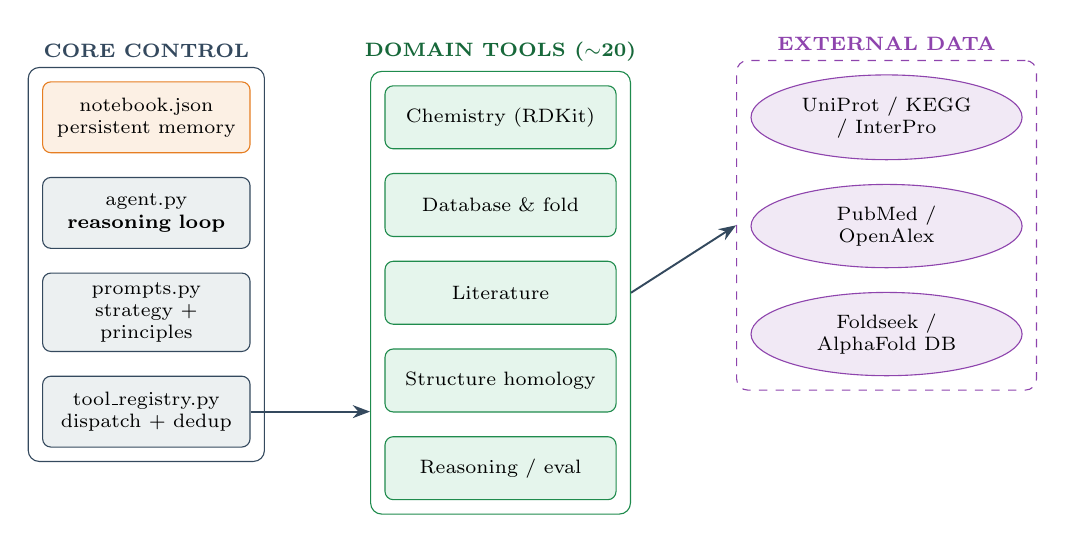
\begin{tikzpicture}[node distance=3mm]
    % Core control
    \node[core] (agent) {agent.py\\\textbf{reasoning loop}};
    \node[core, below=of agent] (prompts) {prompts.py\\strategy + principles};
    \node[core, below=of prompts] (reg) {tool\_registry.py\\dispatch + dedup};
    \node[core, draw=accentorange, fill=accentorange!12, above=of agent] (nb)
         {notebook.json\\persistent memory};
    \begin{scope}[on background layer]
      \node[draw=darkgray, rounded corners, fit=(nb)(agent)(prompts)(reg),
            inner sep=5pt, label={[font=\scriptsize\bfseries, darkgray]above:CORE CONTROL}] (corebox) {};
    \end{scope}

    % Tools
    \node[toolb, right=1.7cm of nb]    (t1) {Chemistry (RDKit)};
    \node[toolb, below=of t1]          (t2) {Database \& fold};
    \node[toolb, below=of t2]          (t3) {Literature};
    \node[toolb, below=of t3]          (t4) {Structure homology};
    \node[toolb, below=of t4]          (t5) {Reasoning / eval};
    \begin{scope}[on background layer]
      \node[draw=accentgreen!80!black, rounded corners, fit=(t1)(t5),
            inner sep=5pt, label={[font=\scriptsize\bfseries, accentgreen!60!black]above:DOMAIN TOOLS ($\sim$20)}] (toolbox) {};
    \end{scope}

    % APIs
    \node[apib, right=1.7cm of t1] (a1) {UniProt / KEGG / InterPro};
    \node[apib, below=of a1]       (a2) {PubMed / OpenAlex};
    \node[apib, below=of a2]       (a3) {Foldseek / AlphaFold DB};
    \begin{scope}[on background layer]
      \node[draw=softpurple, rounded corners, dashed, fit=(a1)(a3),
            inner sep=5pt, label={[font=\scriptsize\bfseries, softpurple]above:EXTERNAL DATA}] (apibox) {};
    \end{scope}

    \draw[arr] (reg) -- (toolbox.west |- reg);
    \draw[arr] (toolbox.east) -- (apibox.west);
  \end{tikzpicture}
  \end{center}
  \vspace{-1mm}
  {\footnotesize Tools return a uniform \texttt{\{status, summary, data, suggestions\}};
  parallel-safe tools run concurrently (thread pool); near-duplicate searches are cached;
  old tool outputs are pruned to keep the prompt bounded.}
\end{frame}

% ── 5. The reasoning loop ───────────────────────────────────
\begin{frame}{The reasoning loop (ReAct + reflection)}
  \begin{columns}[c]
    \begin{column}{0.42\textwidth}
      \centering
      \includegraphics[height=0.78\textheight]{../enzyme_design_agent/summary/agent_loop_pro.png}
    \end{column}
    \begin{column}{0.58\textwidth}
      \footnotesize
      Each iteration:
      \begin{enumerate}\setlength\itemsep{3pt}
        \item \textbf{State header} injected (iteration, \#candidates, phase)
        \item \textbf{Reflection gate} every 5 iters --- review coverage, re-plan
        \item \textbf{LLM reasons} and emits tool calls (Claude via Argo)
        \item \textbf{Dedup} $\rightarrow$ \textbf{parallel tool execution} $\rightarrow$ results
        \item \textbf{Notebook} updated with synthesized analysis (not raw dumps)
        \item Loop until the agent decides discovery is complete
      \end{enumerate}
      \medskip
      \begin{block}{Guardrails}
        \scriptsize
        \textbf{Critique gate} before evaluation: the agent must justify each
        candidate (correct direction, compatible substrate) --- wrong-reaction
        enzymes are dropped early. \textbf{Context pruning} keeps the prompt from
        ballooning over a long run.
      \end{block}
    \end{column}
  \end{columns}
\end{frame}

% ── 6. How it discovers (pipeline) ──────────────────────────
\begin{frame}{How it discovers enzymes --- the discovery arc}
  \begin{center}
  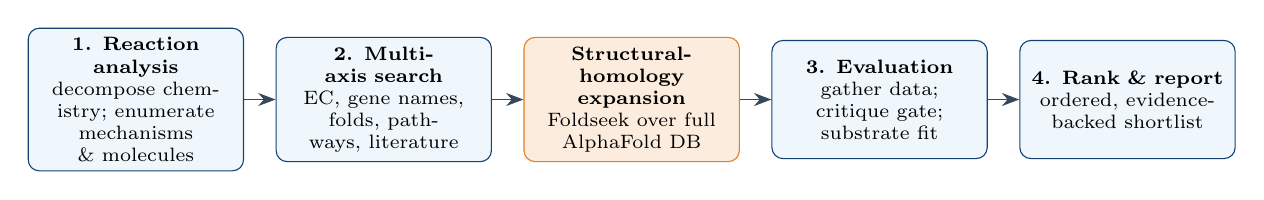
\begin{tikzpicture}[node distance=4mm]
    \node[stage] (s1) {\textbf{1. Reaction analysis}\\\scriptsize decompose chemistry; enumerate mechanisms \& molecules};
    \node[stage, right=of s1] (s2) {\textbf{2. Multi-axis search}\\\scriptsize EC, gene names, folds, pathways, literature};
    \node[stage, right=of s2, fill=accentorange!15, draw=accentorange] (s3) {\textbf{Structural-homology expansion}\\\scriptsize Foldseek over full AlphaFold DB};
    \node[stage, right=of s3] (s4) {\textbf{3. Evaluation}\\\scriptsize gather data; critique gate; substrate fit};
    \node[stage, right=of s4] (s5) {\textbf{4. Rank \& report}\\\scriptsize ordered, evidence-backed shortlist};
    \draw[arr] (s1)--(s2); \draw[arr] (s2)--(s3); \draw[arr] (s3)--(s4); \draw[arr] (s4)--(s5);
  \end{tikzpicture}
  \end{center}
  \vfill
  \begin{columns}[T]
    \begin{column}{0.5\textwidth}
      \footnotesize
      \textbf{Recall (broad, by mechanism):} stages 1--2 plus structural
      expansion cast a wide net across \emph{every} biological context where the
      target bond occurs --- not just the obvious EC class.
    \end{column}
    \begin{column}{0.5\textwidth}
      \footnotesize
      \textbf{Precision (narrow, by fit):} stages 3--4 reason over per-substrate
      chemistry, domain architecture, and evidence to order candidates ---
      \emph{no hand-tuned composite score}.
    \end{column}
  \end{columns}
\end{frame}

% ── 7. The three mechanisms that find hidden enzymes ────────
\begin{frame}{Three mechanisms that surface \emph{hidden} catalysts}
  \begin{block}{Molecule enumeration \hfill {\normalfont\scriptsize(reaction analysis)}}
    \footnotesize
    Exhaustively list every biomolecule that contains the target bond (amino acids,
    cofactors, cell wall, siderophores, antibiotics, biopolymers, \dots). Each
    becomes a search term. \textbf{Coverage emerges from chemistry --- no answer
    enzymes are hardcoded.}
  \end{block}
  \begin{block}{Reference mining \hfill {\normalfont\scriptsize(literature)}}
    \footnotesize
    Specific gene names usually live in a paper's \emph{full text}, not its abstract.
    \texttt{deep\_literature\_search} follows citation networks --- the referenced
    papers name those enzymes in their own titles, recovering catalysts the LLM never saw in training.
  \end{block}
  \begin{alertblock}{Structural-homology expansion \hfill {\normalfont\scriptsize(structure)}}
    \footnotesize
    From the best candidates, \texttt{find\_structural\_homologs} (Foldseek, full
    AlphaFold DB incl.\ TrEMBL) reaches divergent / unannotated relatives that
    sequence \& keyword search cannot. \textbf{Fold $\neq$ chemistry:} a hit is
    promoted only if its \emph{catalytic domain + residues} are conserved --- not on
    TM-score alone.
  \end{alertblock}
\end{frame}

% ── 8. Worked example ───────────────────────────────────────
\begin{frame}{Worked example: MVAP $\rightarrow$ isopentenyl phosphate}
  \footnotesize
  Query: \emph{find enzymes for the ATP-dependent decarboxylation--dehydration of
  mevalonate-5-phosphate}. One autonomous run discovered
  \textbf{5 mechanistic families, 23 candidates evaluated}.
  \medskip
  \begin{columns}[T]
    \begin{column}{0.6\textwidth}
      \renewcommand{\arraystretch}{1.15}
      \begin{tabular}{@{}p{1.5cm}p{2.2cm}p{2.4cm}@{}}
        \hline
        \textbf{Rank} & \textbf{Enzyme} & \textbf{Why} \\ \hline
        1 & D4GXZ3 \emph{mvaD} & exact reaction + substrate \\
        2--3 & EC 4.2.1.182 dehydratases & perfect substrate match; 1st chemical step \\
        4--6 & EC 4.1.1.33 decarboxylases & same fold; 1-mutation to activity \\
        7+ & UbiD / prFMN, MBD & alt.\ mechanism / partial fit \\ \hline
      \end{tabular}
    \end{column}
    \begin{column}{0.4\textwidth}
      \begin{block}{Two ranking views}
        \scriptsize
        \textbf{Confidence:} direct, well-characterized catalysts first. \\[3pt]
        \textbf{Suitability (explorative):} floats the \emph{substrate-perfect}
        dehydratase family --- the engineering opportunity a confidence ranking buries.
      \end{block}
    \end{column}
  \end{columns}
  \vfill
  \centering\scriptsize\color{darkgray}
  Families span GHMP-kinase, aconitase-X [4Fe-4S], and UbiD radical folds ---
  all reached from the chemistry, each ranked on per-substrate fit + evidence.
\end{frame}

% ── 9. Summary & roadmap ────────────────────────────────────
\begin{frame}{Summary \& what's next}
  \begin{columns}[T]
    \begin{column}{0.52\textwidth}
      \begin{block}{What the framework is}
        \footnotesize
        \begin{itemize}\setlength\itemsep{2pt}
          \item Autonomous ReAct agent: reason $\rightarrow$ search $\rightarrow$ evaluate $\rightarrow$ rank
          \item \textbf{Mechanism-anchored recall} (chemistry, folds, citation networks, structure)
          \item \textbf{Substrate-fit ranking} on grounded cheminformatics facts --- no composite score
          \item Reflection, critique gate, dedup, pruning keep it focused over long runs
        \end{itemize}
      \end{block}
    \end{column}
    \begin{column}{0.48\textwidth}
      \begin{alertblock}{Roadmap}
        \footnotesize
        \begin{itemize}\setlength\itemsep{2pt}
          \item \textbf{Boltz-2 co-folding + NAC geometry}: separate active from
                in-family-\emph{inactive} catalysts (e.g.\ AsbA vs AsbB) ---
                physics is the discriminator structure homology can't provide
          \item Pose-transfer for the top tier; confidence-gated
          \item Benchmark recall under a strict leakage firewall
        \end{itemize}
      \end{alertblock}
    \end{column}
  \end{columns}
  \vfill
  \begin{center}\small\color{deepblue}
  Search broadly by mechanism; rank precisely by substrate fit; confirm with physics.
  \end{center}
\end{frame}

\end{document}
